\section{实证评价}
\subsection{评价对象}
科研系统可以交付答案、程序、实验方案或一篇论文，评价不能只依据同一个文本分数。
文献回答需要检查来源支持，程序任务需要核对执行结果，开放研究还涉及选题、对照和解释。
表\ref{tab:benchmarks}列出几种常用评价工作的对象；它们回答不同问题，并没有形成一个统一的科研能力量尺。

ScienceAgentBench从44篇同行评审论文中提取102项数据驱动任务，要求系统生成独立程序并保存输出\cite{sciencebench}。
有效执行率（valid execution rate，VER）检查能否执行并产生规定输出；任务成功率（success rate，SR）进一步检查是否达到各项任务的标准。
这一差别使实验中一个常被忽略的事实可见：程序已经运行，任务仍可能没有完成。
基准针对的是研究工作流中的具体计算任务，而非一项完整发现。

RE-Bench采用7个开放机器学习研究工程环境，并引入人类专家尝试\cite{rebench}。
其人与代理的相对表现随时间预算改变：代理在短预算下表现较强，而人类在更长预算下取得更明显的后续收益。
这一结果提醒研究者，“超过专家”必须与任务、时间和尝试分配一起报告。
代理快速搜索若干方案与专家长期改进同一研究，并不是可以不计资源直接比较的活动。

\begin{table*}[t]\centering\tabletext
\caption{科研评价工作的任务及测量内容。}
\label{tab:benchmarks}
\begin{tabularx}{\textwidth}{@{}L{39mm}L{48mm}Y@{}}\toprule
\textbf{评价工作} & \textbf{任务材料} & \textbf{主要测量内容}\\\midrule
\tabname{PaperQA2 / LitQA2}{paperqa} & 检索、综合与矛盾识别 & 回答质量、来源支持及专家比较\\[5pt]
\tabname{ScienceAgentBench}{sciencebench} & 44篇论文中的102项任务 & VER、SR、代码相似度及费用\\[5pt]
\tabname{RE-Bench}{rebench} & 7个研究工程环境 & 不同时间预算下的任务收益\\[5pt]
\tabname{MAST}{mast} & 多代理轨迹及失败案例 & 规范、协调和核验环节的失败类型\\[5pt]
科研过程审计\cite{pitfalls} & 100个受控审计案例 & 方法学缺陷识别准确率\\\bottomrule
\end{tabularx}
\tabnote{注：VER为有效执行率，SR为任务成功率。各工作的任务、预算及评分定义不同，成绩不可直接合并。}
\end{table*}

\subsection{执行反馈的实证表现}
图\ref{fig:sciencebench}重绘ScienceAgentBench中两个模型在三种框架下的结果。
直接生成（Direct）提供简单参照，Self-Debug允许依据执行反馈修订，OpenHands CodeAct提供更广的交互动作。
原协议对每项任务独立运行三次，依次按SR、VER、CodeBERTScore和较低费用择优，再汇总入选运行。
这些数值因此反映择优后的表现，不是一次运行的均值。

在无专家知识的设置中，Claude 3.5 Sonnet与Self-Debug结合的VER为92.2\%，SR却为32.4\%；GPT-4o对应为83.3\%与22.6\%\cite{sciencebench}。
两者分别相差59.8和60.7个百分点。
仅有汇总数据还不能把差距归因到某一种错误，却足以否定“程序能运行就完成了任务”的判断。
执行反馈能排除一部分实现问题，数据处理和科学目标仍需要单独检查。

资源投入也没有与成功率形成简单的单调关系。
Claude 3.5 Sonnet使用OpenHands时，平均API费用为0.958美元、SR为21.6\%；Self-Debug对应为0.057美元和32.4\%\cite{sciencebench}。
这里比较的是相同模型、相同基准下的框架配置，说明更大的动作空间不一定更容易被有效利用。
它支持将简单反馈方案列为基线，尚不能推广成某一框架在所有任务中更优。
同样，这组实验比较的是代理框架，并未直接分离多代理角色协作的效果。

\begin{figure*}[t]\centering
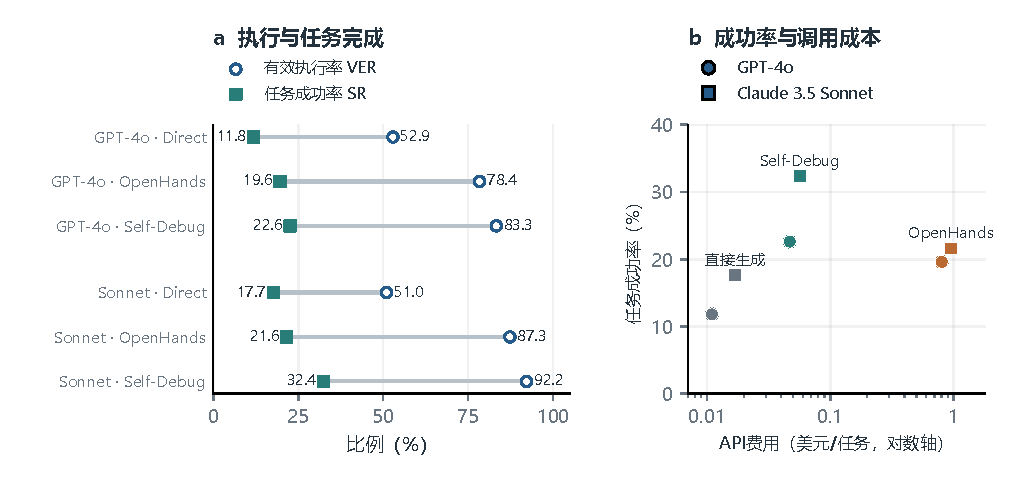
\includegraphics[width=\textwidth]{figures/review-sciencebench.pdf}
\caption{ScienceAgentBench中六组配置的执行、成功与费用。数据取自文献\cite{sciencebench}表3（v3，PDF第8页），均不提供专家知识，共102项任务，每项三次独立运行后择优。
(a) VER与SR；(b) SR与平均API调用费用，对数横轴。模型和美元费用对应原报告时期；点表示表3汇总结果，不是三次运行均值。}
\label{fig:sciencebench}\end{figure*}

\subsection{科研过程审计}
MAST将多代理失败整理为规范与系统设计、主体间失配以及任务核验等类别\cite{mast}。
这类过程分类有助于定位问题：目标理解错误、交接丢失条件和过早结束任务，可能需要完全不同的修正。
只看最终论文，往往无法区分这些原因。

Luo等进一步考察自动科研中的基准选择偏差、数据泄漏、指标误用、事后选择和数据替换或编造等缺陷\cite{pitfalls}。
在其100个正负均衡案例上，审计模型仅阅读论文时总体准确率为55\%，同时获得日志和代码后提高到82\%。
图\ref{fig:audit}以各类识别正确的案例数展示这一变化。
数据泄漏从11/20提高到18/20，事后选择从10/20提高到14/20，说明过程材料的帮助在不同问题上也有差异。

\begin{figure*}[t]\centering
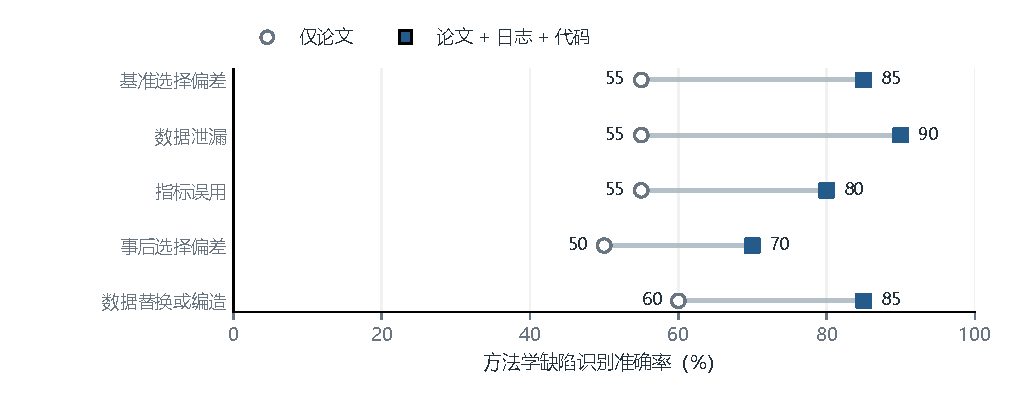
\includegraphics[width=\textwidth]{figures/review-audit.pdf}
\caption{补充过程材料后的缺陷识别。由文献\cite{pitfalls}第6.2节及表11（v2，PDF第16--18页）中的准确率换算为正确案例数；每类20例，阳性、阴性各10例，部分缺陷为原作者受控注入。
审计模型为gemini-2.5-flash-preview-05-20；日志与代码同时加入，未分别估计二者贡献。}
\label{fig:audit}\end{figure*}

这一实验支持提供过程材料，却没有测量真实科研中缺陷有多常见。
案例数量、受控注入和正负比例规定了结果的解释范围；图中也不据此补出总体发生率或不确定区间。
更值得注意的是，论文与过程记录能够回答的问题不同。
前者陈述最终采用的分析，后者可能揭示筛掉了哪些尝试、何时查看过测试结果、训练和测试数据究竟如何使用。
自动化越深入，这种差别越有可能影响对研究的判断。

\subsection{协作增益的归因分析}
若要识别协作贡献，单代理基线应具有相应的检索、执行和重试机会，并尽量匹配模型、工具、预算与人工帮助。
否则，多代理系统获得的提升虽是系统层面的真实差异，却未必来自角色分工。
消融还需要说明资源如何重新分配：删除检查者并同时减少调用次数，不能单独回答检查角色是否必要。

更有针对性的比较是保留总预算后合并角色，或保留角色数量但改变检查者能访问的材料。
前者观察分工与通信是否值得，后者观察检查的信息来源是否产生增益。
对长期任务，还可检查系统在一项关键判断被推翻后，能否找出受影响的后续实验。
这些评价比单独增加一个最终答案分数更难，但也更贴近科研协作实际要解决的问题。
